\section{Intégration du jeu}
\subsection{Jeu}
\begin{figure}[h!]
	\centering
	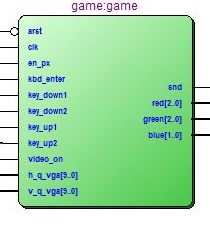
\includegraphics[scale=1.0]{images/game.jpg}
	\caption{Entité game}
	\label{fig:game}
\end{figure}
L'entité \emph{game} a pour rôle d'instancier tous les éléments nécessaires au jeu. L'entité \emph{clkdiv} est instancié pour obtenir un enable permettant de gérer la vitesse de mise à jour du jeu en lui même, et un autre enable pour gérer la vitesse des raquettes uniquement. Les autres entités instanciées sont les suivantes \emph{player} (gestion du joueur), \emph{sounds} (génération des sons de collision), \emph{ball} (gestion de la balle), \emph{score}, \emph{game\_gen} (génération des éléments du jeu via les signaux de couleurs du VGA), \emph{game\_state} (état du jeu).
\begin{figure}[h!]
	\centering
	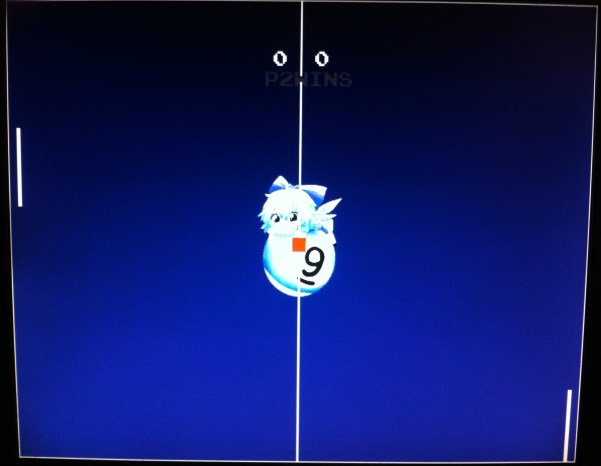
\includegraphics[scale=0.5]{images/IMG_1015.jpg}
	\caption{Photo du jeu en fonctionnement}
	\label{fig:photogame}
\end{figure}

\newpage
\subsection{Éléments du jeu}
\begin{figure}[h!]
	\centering
	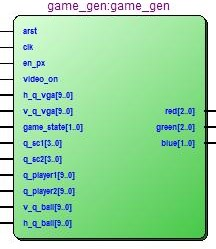
\includegraphics[scale=1.0]{images/gamegen.jpg}
	\caption{Entité game\_gen}
	\label{fig:gamegen}
\end{figure}

La génération des éléments du jeu et des couleurs s'effectue grâce à l'entité \emph{game\_gen}. Celle-ci possède en sortie les 3 signaux de couleurs nécessaires à l'affichage VGA \emph{red}, \emph{green} et \emph{blue}. Les entrées sont principalement les différents compteurs de position (\emph{h\_x\_vga},  \emph{q\_scx}, \emph{q\_player1} et \emph{x\_q\_ball}.\\

Le signal \emph{color\_gen} permet de coder la priorité d'affichage des différents éléments du jeu. Les éléments à afficher sont les suivants (du plus important au moins important) :
\begin{description}
\item[win\_gen] texte "P1/2WINS"
\item[start\_gen] texte "PRESS ENTER"
\item[ball\_gen] balle
\item[player\_gen] joueur
\item[score2\_gen] affichage score joueur2
\item[score1\_gen] affichage score joueur1
\item[bg\_gen] affichage background
\item[BLACK] affichage couleur noire (lorsque les compteurs de pixels ne sont plus dans la zone active définie par \emph{video\_on})
\end{description}

\newpage
\subsection{État du jeu}
\begin{figure}[h!]
	\centering
	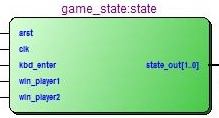
\includegraphics[scale=1.0]{images/gamestate.jpg}
	\caption{Entité game\_state}
	\label{fig:gamestate}
\end{figure}
La gestion de l'état dans lequel se trouve le jeu se trouve dans l'entité \emph{game\_state}. Celle-ci est une machine
d'état décrite par le schéma suivant (\emph{game\_state} état actuel de la machine d'état, \emph{kbd\_enter\_new} état actuel de la touche entrée du clavier, \emph{kbd\_enter\_old} ancien état de la touche entrée du clavier, \emph{win\_player1} état de victoire du joueur 1, \emph{win\_player2} état de victoire du joueur 2):
\begin{figure}[h!]
	\centering
	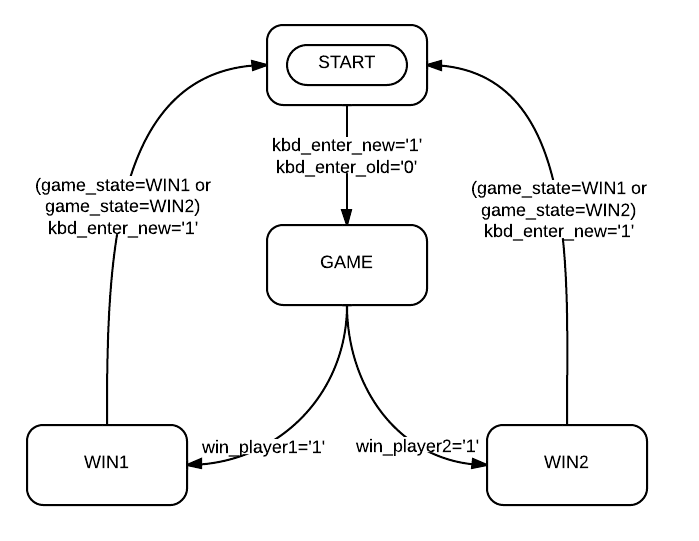
\includegraphics[scale=0.5]{images/BasicStateDiagram.png}
	\caption{Schéma de la machine d'état}
	\label{fig:statemachine}
\end{figure}

Les états possibles sont les suivants :
\begin{description}
\item[START] Affichage du texte "PRESS START", attente de l'appui sur la touche entrée pour lancer le jeu
\item[GAME] Jeu en fonctionnement
\item[WIN1] Le player1 a gagné, affichage du texte "P1WINS", attente de l'appui sur la touche entrée pour revenir à l'écran start
\item[WIN2] le player2 a gagné, affichage du texte "P2WINS", attente de l'appui sur la touche entrée pour revenir à l'écran start
\end{description}

\newpage
\subsection{Joueur}
\begin{figure}[h!]
	\centering
	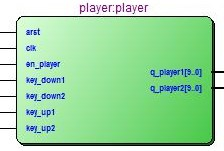
\includegraphics[scale=1.0]{images/player.jpg}
	\caption{Entité player}
	\label{fig:player}
\end{figure}

Un joueur est représenté par sa raquette. La gestion des joueurs est effectuée dans l'entité \emph{player} qui contient un compteur de position verticale pour chaque joueur. Ce compteur (instanciation de l'entité \emph{cnt\_player}) peut compter de 0 (haut de l'écran) jusqu'à \emph{zone active verticale} - \emph{hauteur du joueur} (bas de l'écran).\\

\begin{figure}[h!]
	\centering
	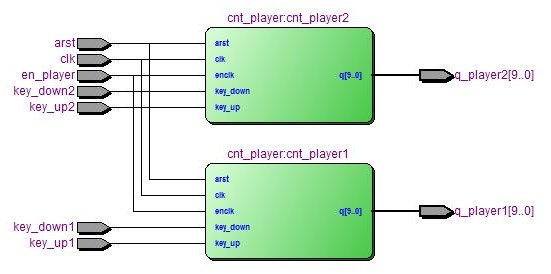
\includegraphics[scale=1.0]{images/player_player.jpg}
	\caption{Schéma interne de l'entité player}
	\label{fig:playerplayer}
\end{figure}

L'entité \emph{cnt\_player} gérant la position d'un joueur est un compteur pouvant s'incrémenter ou se décrémenter en fonction des signaux \emph{key\_up} et \emph{key\_down}. Ces signaux proviennent de l'état de boutons contrôlant les raquettes des joueurs, boutons provenant dans notre cas du clavier interfacé avec le FPGA. Si la valeur maximum(ou minimum) du compteur est atteinte, le compteur reste à cette valeur si le signal \emph{key\_down} (ou \emph{key\_up}) est actif.\\

L'entité \emph{player} possède en sortie les signaux \emph{q\_player1} et \emph{q\_player2} provenant des compteurs de position des joueurs.

\newpage
\subsection{Balle}
\begin{figure}[h!]
	\centering
	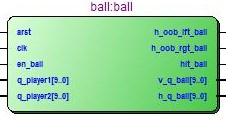
\includegraphics[scale=1.0]{images/ball.jpg}
	\caption{Entité ball}
	\label{fig:ball}
\end{figure}

La balle est le seul élément du jeu à se déplacer en deux dimensions. Sa gestion est effectuée dans l'entité \emph{ball} et  fait appel à trois paramètres : position, vitesse et angle de déplacement. Dans les premières versions du projet, la position était le seul paramètre variable (valeurs des compteurs de position). Par la suite, la vitesse et l'angle de déplacement sont devenus des variables.\\

Comme la balle se déplace en deux dimensions, il a fallu trouver un système permettant de gérer les déplacements horizontaux et verticaux simultanément. Les compteurs se sont immédiatement imposés comme le meilleur moyen de gérer une position, leurs valeurs respectives donnant la position de la balle a un instant précis. La position future de la balle dépend de sa position actuelle et de différents paramètres, notamment le choc contre une raquette ou la sortie de l'écran ou encore le fait que la balle soit montante ou descendante. Les compteurs devaient donc adapter leur comportement en fonction de ces paramètres.\\

Au départ, il s'agissait de deux compteurs basiques à deux modes : incrémentation et  décrémentation. Leurs comportements étant différents ils possédaient deux architectures différentes : une pour la position horizontale et une pour la position verticale. Dans la dernière version il s'agit toujours d'un compteur à deux modes, l'entité \emph{cnt\_ball}, cependant le mode de fonctionnement (horizontal ou vertical) n'est plus géré par deux architectures différentes mais par un generic, \emph{CNT\_MODE} (peut prendre les valeurs (\emph{CNT\_MODE\_H} ou \emph{CNT\_MODE\_V}. Ce compteur est instancié deux fois, une pour la position horizontale de la balle, et l'autre pour la position verticale.\\

Les génériques MAX et MIN permettent de définir les valeurs extrêmes prises par q, sortie du compteur. Il faut garder à l'esprit que du fait de la multiple instanciation, les valeurs de MAX et de MIN sont définies différemment selon le mode du compteur : vertical ou horizontal.\\

Le signal \emph{mode} dans \emph{cnt\_ball} permet de contrôler le sens de variation des compteurs : incrémentation ou décrémentation. Le \emph{spd\_mod} permet de contrôler la vitesse du compteur : selon sa valeur le compteur est incrémenté ou décrémenté, d'une valeur plus ou moins élevé.\\

L'angle de rebond n'est pas une variabe, il est calculé grâce à un système de zone de collision et appliqué grâce à une combinaison des \emph{spd\_mod} sur les compteurs verticaux et horizontaux. Le comportement de la balle dépend de l'endroit où elle touche la raquette. Pour cela, on utilise les signaux \emph{hit\_rgt\_area} et \emph{hit\_left\_area} qui influe sur le comportement de \emph{spd\_mod}. Ces signaux sont des entrées de l'entité, ils sont générés dans l'entité \emph{ball}.\\

\newpage
\begin{figure}[h!]
	\centering
	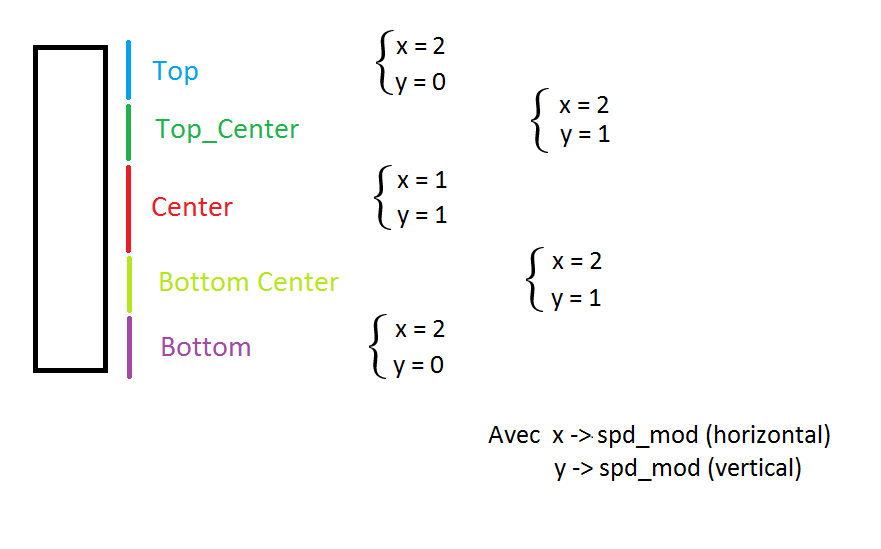
\includegraphics[scale=0.5]{images/collisions.png}
	\caption{Schéma zones de collision et effets sur la balle}
	\label{fig:collisions}
\end{figure}

Les signaux \emph{oob\_rgt} et \emph{oob\_lft} sont utilisés afin de savoir si la balle est sortie de l'écran horizontalement et permet donc de savoir si un des joueurs à marqué un point.

\newpage
\subsection{Scores}
\begin{figure}[h!]
	\centering
	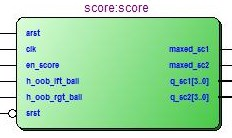
\includegraphics[scale=1.0]{images/score.jpg}
	\caption{Entité score}
	\label{fig:score}
\end{figure}

La gestion des scores est effectuée dans l'entité \emph{score} qui possède en entrée le signal d'enable \emph{en\_score} (vitesse de mise à jour du jeu), des signaux permettant de savoir si la balle est sortie de l'écran à droite ou à gauche \emph{h\_oob\_rgt\_ball} et \emph{h\_oob\_lft\_ball}. Les sorties sont des vecteurs permettant de connaître le score \emph{q\_sc1} et \emph{q\_sc2}, et deux signaux permettant de savoir si le score a atteint sa valeur max \emph{maxed\_sc1} et \emph{maxed\_sc2}.\\

\begin{figure}[h!]
	\centering
	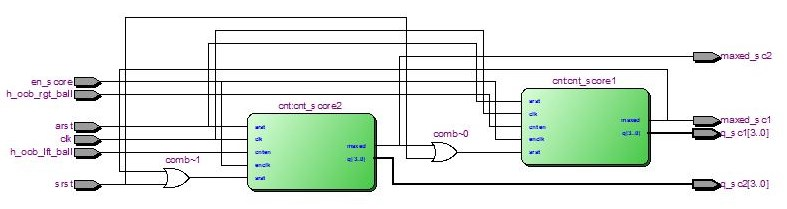
\includegraphics[scale=0.75]{images/scorein.jpg}
	\caption{Schéma interne de l'entité score}
	\label{fig:scorein}
\end{figure}
L'architecture de cette entité contient l'instanciation de deux compteurs (entité \emph{cnt}) permettant de compter de 0 jusqu'à \emph{MAX\_SCORE}. Ces compteurs sont autorisés à compter lorsque le joueur correspondant à marqué un point (\emph{h\_oob\_rgt\_ball} à l'état haut ou \emph{h\_oob\_lft\_ball} à l'état haut). Enfin, le reset synchrone des compteurs est activé lorsqu'un des joueurs à atteint le score max et/ou que le jeu n'est pas dans l'état \emph{GAME} (voir partie sur la gestion des états du jeu).

\newpage
\subsection{Génération de sons}
\begin{figure}[h!]
	\centering
	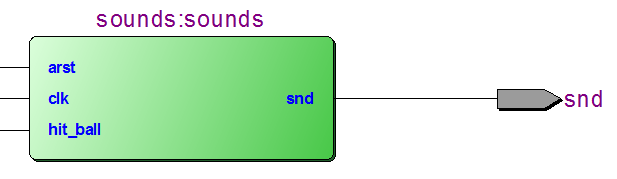
\includegraphics[scale=0.75]{images/soundsschem.png}
	\caption{Schéma entité sounds}
	\label{fig:soundschem}
\end{figure}

Le haut parleur que nous utilisons possède une impédance de 8 Ohms et une puissance maximale de 0.3W. Nous sortons du 3.3V LVTTL avec un courant de 8 mA sur le pin sur lequel nous branchons le haut-parleur.\\

Pour générer un son, nous devons envoyer un signal périodique possédant une fréquence contenue dans les fréquences audibles au haut-parleur. Pour ce faire nous avons instancié l'entité \emph{clkdiv} afin de générer un \emph{enable} permettant de faire fonctionner d'autres signaux à une certaine fréquence. Soit \emph{BUMP\_SOUND}, fréquence souhaitée en utilisant le diviseur d'horloge. Le son est généré en inversant l'état du signal \emph{bumpsnd} à chaque impulsion \emph{enable}, la fréquence sortie sera donc le double de celle précisée dans la constant \emph{BUMP\_SOUND}.\\

Une fois le son généré, nous souhaitons pouvoir le maintenir, pour cela nous utilisons un autre diviseur d'horloge utilisant une fréquence \emph{HOLD\_SOUND}, dont la période correspondante est le temps de maintien du son. Nous autorisons ensuite à sortir le signal \emph{bumpsnd} de l'entité lorsqu'une collision entre la balle et une raquette intervient (\emph{hold\_hit\_ball}='1') et tant que l'enable du diviseur d'horloge de maintien du son ne passe pas à l'état bas.

\begin{figure}[h!]
	\centering
	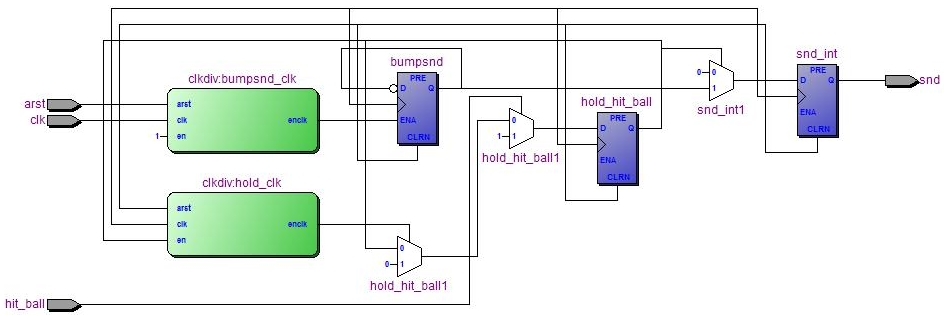
\includegraphics[scale=0.70]{images/soundsschem2.jpg}
	\caption{Schéma interne entité sounds}
	\label{fig:soundschem2}
\end{figure}

\newpage
